\newpage\part{Flash Cards}

\section{Farmaci del SNC e del SNP}

\begin{tikzpicture}
	\tikzset{level distance=90pt,frontier/.style={distance from root=370pt}} 
	\Tree
	[.SNC
		[.Periferico
			[.Sensitivo ]
			[.Autonomo
		 		[ .{Simpatico\\ (toraco--addominale)} {gangli pre e para--vertebrali} ]
				[ .{Parasimpatico \\(nervi crani e sacrale)} {nell'intima degli organi} ]
			]
			[.Gastroenterico {plessi mioenterici (Auerbach) e\\ sottomucosi (Meissner)}
			]
		]
		[.Centrale ]
	]
\end{tikzpicture}

\begin{tikzpicture}
	\tikzset{level 1/.style={level distance=150pt}}
	\Tree
	[.{Neurotrasmettitori\\ SNP}
		 [.\node(acetilcolina){acetilcolina}; {recettori colinergici} ]
		 [.noradrenalina {recettori adrenergici} ]
		 [.\node(serotonina){serotonina\\5-HT 5-idrossitriptamina}; {recettori serotoninergici} ]
		 [.{monossido d'azoto (NO)} ] 
		 [.purine ]
	]
	\begin{scope}[yshift=-9em]
	\Tree
	[.\node(snc){Neurotrasmettitori\\ SNC};
		[.dopamina {recettori dopaminergici} ]
		Glutammato
		GABA
	]
	\end{scope}
	\draw[drawarrow] (snc.east) to[in=180,out=40] (acetilcolina.west)
		(snc.east) to[in=180,out=0] (serotonina.west);
\end{tikzpicture}

\subsection{Acetilcolina}

\begin{tikzpicture}
	\tikzset{level 1/.style={level distance=150pt}}
	\Tree
	[.localizzazione {tutte le fibre pregangliali sia para che orto\\ nicotiniche} {parasimpatiche post gangliali (quasi tutte).\\ muscariniche} {ghiandole sudoripare (simpatico)\\ muscariniche} {giunzione neuromuscolare\\ nicotiniche} ]
\end{tikzpicture}

\begin{tikzpicture}
	\tikzset{level 2/.style={level distance=130pt}, level 3/.style={level distance=120pt}}
	\Tree
	[.Sintesi
		[.colina \edge node[smallfont,yshift=5pt,xshift=5.4em]{entra nel neurone} node[smallfont,yshift=-5pt,xshift=5.4em]{tappa limitante};
			[.{acetilCOA + colina} \edge node[smallfont,yshift=-5pt,xshift=5em]{acetiltrasferasi} node[smallfont,yshift=5pt,xshift=5em]{colina}; acetilcolina ]
		]
	]
\end{tikzpicture}

\begin{tikzpicture}
	\tikzset{level 2/.style={level distance=130pt}}
	\Tree
	[.Degradazione
		[.acetilcolina \edge node[smallfont, yshift=-5pt,xshift=5.5em]{acetilcolinesterasi}; {acetato + colina} ]
	]
\end{tikzpicture}

\begin{tikzpicture}
	\Tree
	[.Liberazione 
		[.{Ca${}^{2+}$ + VAMP/SNAPS}
			[.{fusione vescicole con\\ membrana neuronale} esocitosi
			]
		]
	]
\end{tikzpicture}

\begin{tikzpicture}
	\tikzstyle{cwhite}=[circle,shadedraw=yellow];
	\shade[ball color=yellow] node (ach) {\small Ach} circle[radius=.45];
	\draw (ach) -- +(.7,.7) node(vamp){} arc [start angle=225, end angle=270, radius=6pt]  (.7,.7) arc [start angle=225, end angle=180, radius=6pt];
	\draw (2,2) arc [start angle=45, end angle=0, radius=3cm] node[midway,above,sloped]{\tiny spazio sinaptico} ;
	\draw (2,2) 
		arc [start angle=45, end angle=60, radius=3cm] node(a){} 
		node[above right=2pt and 2pt of a] {\tiny Canale Ca${}^{2+}$}
		(a) arc [start angle=140, end angle=120, radius=1cm]
		(a) arc [start angle=140, end angle=160, radius=1cm];
	\path (2,2) arc [start angle=45, end angle=65, radius=3cm] node(b){};
	\draw (b) arc [start angle=-50, end angle=-30, radius=1cm]
		(b) arc [start angle=-50, end angle=-70, radius=1cm]
		(b) arc [start angle=65, end angle=80, radius=3cm];
	\draw (2,2) -- (1.3,1.3);
	\filldraw (1.3,1.3) circle[radius=3pt] node(snap){};
	\draw[->, shorten <=0pt,shorten >=2pt] (vamp)--(snap) node[midway,above,circle,draw,,yshift=3pt,xshift=-8pt]{\tiny 2};
	\draw[->, shorten <=0pt,shorten >=2pt] (ach) to[out=-20,in=225] node[midway,below,circle,draw,yshift=-5pt]{\tiny 3}  (4,1) ;
	\draw[->, shorten <=2pt,shorten >=6pt](3,3.5) to[out=205,in=90] node[near end,above,circle,draw,yshift=15pt]{\tiny 1}  node[very near end,above,yshift=15pt,xshift=-2pt]{\tiny Ca${}^{2+}$} (ach) ;
	\node at (1,.4) {\tiny VAMP};
	\node at (1.9,1.3) {\tiny SNAP};
\end{tikzpicture}

\begin{tikzpicture}
	\Tree
	[.Effetti
		[.{$\uparrow$permeabilit\`a ai cationi\\ Na${}^+$, K${}^+$, Ca${}^{2+}$}
			[.depolarizzazione
				[.{fibre post sinaptiche} PdA ]
				[.{fibre muscolari} {generazione potenziale\\ di placca}
				]
			]
		]
	]
\end{tikzpicture}

\begin{tikzpicture}
	\tikzset{level 1/.style={level distance=80pt},level 2/.style={level distance=140pt},level 3/.style={level distance=140pt}}
	\Tree
	[.{Recettore colinergico}
		[.{muscarinico\\ (metabotropo)}
			[.{M${}_1$ eccitatorio $\uparrow\text{IP}_3, \uparrow\text{DAG},\uparrow\text{Ca}^{2+}$} {SNC, simpatico post--gangliare,\\ cellule parietali dello stomaco}
			]
			[.{M${}_2$ inibitorio $\downarrow$cAMP } {cuore, endotelio dei vasi}
			]
			[.{M${}_3$ eccitatorio $\uparrow\text{IP}_3, \uparrow\text{DAG},\uparrow\text{Ca}^{2+}$} {ghiandole esocrine, muscolo liscio,\\ endotelio dei vasi}
			]
			[.{M${}_4$ come $\text{M}_2$} {SNC}
			]
			[.{M${}_5$  come $\text{M}_1$} {endotelio vasale, cervello, SNC}
			]
		]
		[.{nicotinico\\ (ionotropo)}
			[.{N${}_\text{N}$ gangliare} {para e ortosimpatico gangliare} ]
			[.{N${}_\text{M}$ muscolare} {giunzione\\ neuromuscolare} ]
		]
	]
\end{tikzpicture}

\subsubsection{Agonisti colinergici}

\begin{tikzpicture}
	\begin{scope}
	\tikzset{
		level distance=80pt,
		level 1/.style={level distance=70pt},
		level 2/.style={level distance=70pt},
		frontier/.style={distance from root=400pt} 
	}
	\Tree
	[.\node(main){Tipo}; 
		[.diretti
			[.{attivano recettori} 
				[.{esteri della colina} 
					\node(ach){acetilcolina };
					metacolina
					carbacolo
					\node[farmaco](beta){betanecolo};
				]
				[.alcaloidi
					[.muscarinici
						muscarina
						\node[farmaco]{pilocarpina};
					]
					[.nitotinici \node[farmaco]{nicotina}; ]				
				]
			]
		]
		[.indiretti
			[.\node(AchEI){inibitori AchE}; 
			]
		]
	]	
	\node[right=5pt of ach] (achn) {};
	\node[right=5pt of beta] (betan) {};
	\draw[drawarrow] (achn) -- (betan) node[midway,above,sloped] {\tiny $\uparrow$resist. idrolisi e quindi durata azione};
\end{scope}
\begin{scope}[yshift=-14em]
	\Tree
	[.\node(AchEIa){inibitori AchE};
		[.carbammati 
			[.\node[farmaco]{neostigmina\\ fisostigmina\footnotemark}; 
				[.{legame covalente con AchE} {idrolisi in ore}
				]
			]
		]
		[.{alcool+gruppo N quaternario}
			[.\node[farmaco]{edrofonio}; 
				[.{legame idrogeno\\ o ionico con AchE} {idrolisi in minuti}
				]
			]
		]
		[.organofosfati
			[.\node[farmaco](ecotiopato){ecotipato};
				[.\node(fAchE){fosforilazione AchE}; \node(idro){idrolisi in giorni};
				]
			]
			\node(somar){somar\\ (gas nervino)};
		]
	]		
	\draw[drawarrow] (somar) to[out=0,in=180] (fAchE);
	\node[chartnode,below=1em of fAchE] (invec) {invecchiamento\\rottura legame O-P\\ con raffozamento\\ legame con AchE}; 
	\node[chartnode,below=1em of idro] (pral) {pralidossina pu\`o\\ scindere la\\ fosforilazione};
	\draw[drawarrow] (pral)--(fAchE) node[midway,above,sloped] {\tiny qui si};
	\draw[drawarrow] (pral)--(invec) node[midway,above,sloped] {\tiny qui no};
	\node[below right=8pt and 5pt of somar] (somary) {};
	\node[above=9em of somary] (neox) {};
	\draw[drawarrow] (neox) -- (somary) node[midway,above,sloped] {\tiny $\uparrow$durata azione};
	\draw[drawarrow] (AchEI.south) to[out=-90,in=90] (AchEIa);
\end{scope}
\end{tikzpicture}

\footnotetext{Presente nella fava del Calabar}

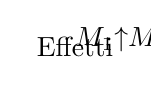
\begin{tikzpicture}
	\tikzset{level distance=120pt, level 2/.style={level distance=150pt}}
	\Tree
	[.\node(sub){Effetti}; 
		[.{SNC ($\text M_1$)} {tremore, ipotermina, $\uparrow$capacità cognittive}	
		]
		[.{occhio ($\text M_3$)}
			{costrizione muscolo sfintere dell'iride (miosi)\\ contrazione muscolo ciliare (accomodamento da vicino)}
		]
		[.{cuore ($\text M_2$)}
			{$\downarrow$frequenza (cronotopo-), $\downarrow$forza (inotropo-),\\ $\downarrow$vel. conduzione (dromotropo-), $\uparrow$periodo refrattario, NAV}
		]
		[.{vasi ($\text M_2$)}
			{vasodilatazione a basse dosi\\ vasocontrazione a alte dosi}
		]
		[.{polmone ($\text M_3$)}
			 {broncocostrizione, $\uparrow$secrezione}
		]
		[.{intestino ($\text M_3$)}
			{$\uparrow$motilit\`a, $\downarrow$ muscolatura sfinteri, $\uparrow$ secrezioni} 
		]
		[.vescica
			 {contrazione destrusore ($\text M_3$), rilascio trigono ($\text M_2$)}
		]
		[.{ghiandole esocrine ($\text M_3$)}
			{$\uparrow$secrezioni}
		]
		[.{giunzione neuromuscolare\\ (indiretti)}
			{basse concentrazioni: $\uparrow$forza contrazione utile \\ se intossicazioni da curaro o miastenia grave\\ alte concentrazioni: fibrillazione fibre muscolari}
		]
	]
\end{tikzpicture}

\begin{tikzpicture}
	\tikzset{frontier/.style={distance from root=350pt}, level 2/.style={level distance=130pt}}
	\Tree
	[.{usi clinici}
		[.\node[farmaco](pilocarpina){pilocarpina};
			[.{xerostomia da\\ sindrome di Sjogren} {$\uparrow$secrezioni salivali}
			]
		]
		[.\node[farmaco](ecotiopato){ecotiopato};
			[.\node(glaucoma){glaucoma};
				{nelle emergenze ad angolo chiuso,\\ agonista muscarinico + inibitore colinesterasi. \\	nel glaucoma cronico ora si usano i $\beta$-bloccanti}
			]
		]
		[.\node[farmaco](betanecolo){betanecolo};
				\node(ritenzione){ritenzioni urinarie e ileo\\ depressione dell'attivit\`a senza ostruzione};
		]
		[.\node[farmaco](neostigmina){neostigmina};
			[.\node(miastenia){miastenia grave};
				{cura e mezzo diagnostico}
			]
		]
		[.\node[farmaco](edofonio){edofonio};
			{tachiaritmia parossistica sopraventricolare\\ in disuso, ora si usa l'adenosina.}
			\node(post){post anestesia per revertire i\\ neurobloccanti muscolari (vedi)};
		]
		[.\node[farmaco](fisostigmina){fisostigmina};
			{intossicazione da farmaci antimuscarinici\\ (intossicazione da atropina)}
		]
	]
	\draw[drawarrow](pilocarpina) to[out=0, in=180] (glaucoma);
	\draw[drawarrow](neostigmina) to[out=0, in=180] (ritenzione);
	\draw[drawarrow](neostigmina) to[out=0, in=180] (post);
	\draw[drawarrow](betanecolo) to[out=0, in=180] (ritenzione);
	\draw[drawarrow](edofonio) to[out=0, in=180] (miastenia);
\end{tikzpicture}

\subsubsection{Antagonisti colinergici}

\begin{tikzpicture}
	\Tree
	[.{antagonisti\\ colinergici}
		[.antimuscarinici 
			[.\node[farmaco]{atropina}; {deriva da Belladonna e\\ Datura Stramonium}
			]
			\node[farmaco]{scopolamina};
		]
		[.antinicotinici 
			[.{bloccanti gangli\\ ganglioplegici} \node[farmaco]{trimetafano}; 
			\node[farmaco]{tossina botulina};
			]
			[.{bloccanti neuromuscolari}
			]
		]
		[.{rigeneratori dell'AchE} \node[farmaco]{pralidossima\footnotemark};
		]
	]
\end{tikzpicture}

\footnotetext{vedi inibitori dell'AchE}

\begin{tikzpicture}
	\Tree
	[.Assorbimento
		[.\node(am3){Ammine III${}^\circ$};
			Transcutaneo
		]
		[.{Ammine IV${}^\circ$}
			\node(intestino){intestino};
			\node(occhio){occhio};
		]
	]
	\draw[drawarrow]
		(am3) to[out=0, in=180] (intestino)
		(am3) to[out=0, in=180] (occhio);
\end{tikzpicture}

\textsc{Antimuscarinici}


\begin{tikzpicture}
	\tikzset{level distance=150pt}
	\Tree
	[.{effetti}
		[.{SNC ($\text M_1$)} {effetto stimolante (-atropina +scopolamina) $\downarrow$tremore Parkinson\\ Parkinson \`e causato da un $\uparrow$ attivit\`a colinergica}
		]
		[.{occhio ($\text M_3$)} {$\uparrow$attivit\`a simpatica $\Rightarrow$ midriasi\\ (belladonna $\equiv$ occhi dilatati\\ incapacit\`a di adattamento\\ visione da vicino)}
		]
		[.{cuore ($\text M_2$)} {tachicardia, blocco vagale, $\downarrow$PR per $\uparrow$dromotropo}
		]
		[.{vasi ($\text M_2/\text M_3$)} incerta ]
		[.{apparato respiratorio ($\text M_3$)} {broncodilatazione, $\downarrow$secrezioni\\ (ma meglio i $\beta$-adrenergici)}
		]
		[.{gastrointestinale ($\text M_3$)} {$\downarrow$secrezioni salivali, minori su tutto il resto} ]
		[.{gh. sudoripare ($\text M_3$)} {soppressione termoregolazione\\ (febbre da atropina)} ]
	]
\end{tikzpicture}

\begin{tikzpicture}
	%\tikzset{level 1/.style={level distance=130pt}}
	\Tree
	[.{usi clinici} 
		[.\node[farmaco](atropina){atropina};
			{malattia di Parkinson}
			{esame oftalmico}
			{pre-operatorio\\ antilaringospasmo}
			{sincope vagale\\ da dolore infarto}
			{ulcera peptidica\\ in disuso}
		]
		[.\node[farmaco]{scopolamina};
			{chinetosi\\ mal di mare}
		]
		[.\node[farmaco]{inatroprio???};
			\node(bpco){BPCO};
		]
		[.\node[farmaco]{oxibutina};
			{tenismo urinario}
		]
		[.\node[farmaco]{pralidossina};
			[.{iperfunzione colinergica}
				{da organofosfati, gas nervino\\ o intossicazione funghi}
			]
		]
	]
\end{tikzpicture}

\begin{tikzpicture}
	\Tree
	[.{Effetti avversi} {febbre da atropina} tachicardia {vasodilatazione con\\ esantema da atropina\\ testa, collo, arti, tronco} ]
\end{tikzpicture}

\textsc{Ganglioplegici}

\begin{tikzpicture}
	\tikzset{level 2/.style={level distance=150pt}}
	\Tree
	[.effetti
		[.SNC {sedazione, tremore}
		]
		[.occhio {perdita accomodamento, effetto su pupilla incerto\\ per innervazione para e orto del m. sfintere}
		]
		[.cardiocirc {$\downarrow$pressione con ipotensione ortostatica marcata}
		]
		[.gasto {$\downarrow$motilit\`a}
		]
		[.urinario {ritardo nella minzione, problemi erezione e eiaculazione}
		]
	]
\end{tikzpicture}

\begin{tikzpicture}
	\tikzset{level 2/.style={level distance=150pt}}
	\Tree
	[.{usi clinici}
		[.\node[farmaco]{trimetafano};
			{ipotensivo nelle anestesie}
		]
		[.\node[farmaco]{tossina botulinica};
			{iniezione intravescicale\\ contro incontinenza}
		]
	]
\end{tikzpicture}

\textsc{Bloccanti neuromuscolari}

\begin{tikzpicture}
	\tikzset{level 3/.style={level distance=150pt}}
	\Tree
	[.{influenza sui muscoli}
		[.{bloccanti neuromuscolari}
			{per indurre paralisi\\ durante gli interventi}
		]
		[.spasmolitici
			[.{per ridurre dolore\\ in varie situazioni}
				{vedi cap. 27 sull'argomento\\ o poi se trattato\\(benzodiazepine, clonidina, antiepilettici, \\ dantrolene (anche contro ipertermia maligna),\\ tossina botulinica)}
			]
		]
	]
\end{tikzpicture}

\begin{tikzpicture}
	\Tree
	[.{bloccanti\\ neuromuscolari}
		[.{non depolarizzanti}
			[.{impediscono l'accesso dell'Ach\\ sul recettore $\text M_M$}
				{tubocuranina\\ (curaro)}
				\node[farmaco]{rocuronio};
			]
		]
		[.depolarizzanti
			[.{eccesso di Ach o simile}
				\node[farmaco]{succinilcolina\\(2 Ach legate tra loro)};
			]
		]
	]
\end{tikzpicture}

\begin{tikzpicture}
	\tikzset{level 2/.style={level distance=130pt}}
	\Tree
	[.Farmacocinetica
		[.assunzione EV ]
		[.metabolismo epatico ]
		[.degradazione \edge node[smallfont,yshift=-5pt,xshift=5em]{AchE (plasma)} node[smallfont,yshift=5pt,xshift=5em]{BuchE (fegato)}; {acido succinico + colina}
		]
	]		
\end{tikzpicture}

Una mutazione del gene che codifica la pseudocolinesterasi plasmatica rende alcuni pazienti pi\`u sensibili a metabolizzare la succinilcolina.

Il n. di dibucaina \`e un parametro per definire tali anomalie e dipende dal fatto che la dibucaina inibisce la pseudoAchE normale per l'80\% mentre l'inibizione \`e solo del 20\% in quella modificata.

\begin{tikzpicture}
	\tikzset{frontier/.style={distance from root=300pt}}
	\Tree
	[.funzionamento
		[.{non depolarizzanti} {stimolo tetanico} ]
		[.depolarizzanti
			[.{fase 1: depolarizzazione} fascicolazione ]
			[.{fase 2: desensibilizzazione} {stimolo tetanico} ]
		]
	]
\end{tikzpicture}

\begin{tikzpicture}
	\Tree
	[.{sequenza tetanica}
		[.{da muscoli piccoli a grandi}
			{m. occhio}
			{m. facciali}
			{m. arti}
			{faringe}
			\node(diaframma){diaframma};
		]
	]
	\node[below right=10pt and 10pt of diaframma] (da) {};
	\node[above=12em of da] (db) {};
	\draw[drawarrow] (da) -- (db) node[midway,above,sloped] {\tiny recupero sequ. inversa};
\end{tikzpicture}

\begin{tikzpicture}
		\tikzset{level distance=150pt}
	\Tree
	[.{effetti avversi}
		iperkalinemia
		{dolore muscolare post operatorio\\ (depolarizzanti)}
		{rilascio istamina e quindi ipotensione}
	]
\end{tikzpicture}

\subsection{Noradrenalina}

\begin{tikzpicture}
	\Tree
	[.noradrenalina 
		[.{simpatiche postgangliari} 
			[.escluso
				{muscolatura vasi renali ($\text D_1$)}
				{ghiandole sudoripare (Ach)}
			]
		]		
	]
\end{tikzpicture}

\begin{tikzpicture}
	\begin{scope}
	\tikzset{level distance=90pt,level 3/.style={level distance=150pt},
	level 2/.style={level distance=130pt},level 4/.style={level distance=60pt}}
	\Tree 
	[.Sintesi 
		[.Tirosina  \edge node[smallfont,yshift=-5pt,xshift=5.5em]{tirosin--idrossilasi} node[smallfont,yshift=5pt,xshift=5.5em]{tappa limitante}; 
			[.{L-Dopa} \edge node[smallfont,yshift=-5pt,xshift=6em]{DOPA decarbossilasi};
				[.\node[farmaco]{dopamina}; \node[dummyc]{};]
			]
		]
	]
	\end{scope}
	\begin{scope}[yshift=-3em,xshift=1em]
	\tikzset{level distance=80pt}
	\Tree
	[.\node[dummyc]{}; 
		[.\node[farmaco]{noradrenalina}; \node[farmaco]{adrenalina};]
	]	
	\end{scope}				
	
\end{tikzpicture}

\begin{tikzpicture}
	\tikzset{level distance=130pt}
	\Tree 
	[.Degradazione
		[.{MAO (mono-ammino ossidasi)\\ in fegato e cellule ?????} ]
		[.{COMT (catecolo O-metiltransferasi)\\ nei neuroni} ]
	]
\end{tikzpicture}

\begin{tikzpicture}
	\tikzset{level 2/.style={level distance=150pt}}
	\Tree	
	[.{Recettore adrenergico\\ (metabotropo \\ a proteine G)} 
		[.{$\alpha$}
			[ .{$\alpha_1\,\text{G}_{\text{q}} \uparrow\text{IP}_3, \uparrow\text{Ca}^{2+}$ (postsinaptiche muscolo liscio)} ]
			[ .{$\alpha_2\,\text{G}_{\text{i}} \downarrow\text{cAMP}$ (presinaptiche muscolo liscio)} ]
		]
		[.{$\beta$}
			[.{$\beta_1\,\text{G}_{\text{s}} \uparrow\text{cAMP}$ (postsinaptiche cuore, adipociti,\\ iuxaglomerulare, epitelio corpi ciliari)} ]
			[.{$\beta_2\,\text{G}_{\text{s}} \uparrow\text{cAMP}$ (postsinaptiche muscolo liscio e cuore)} ]
			[.{$\beta_3\,\text{G}_{\text{s}} \uparrow\text{cAMP}$ (postsinaptiche cuore, adipociti, vescica)} ]		
		]
	]
\end{tikzpicture}

\begin{tabular}{|c|c|c|c|}
\hline 
\textbf{Organo} & \textbf{Tipo} & \textbf{Recettore} & \textbf{Azione} \\ 
\hline\hline 
M. radiale & simpatico & $\alpha_1$ & costrizione \\ 
\hline 
M. circolare & parasimpatico & M${}_3$ & costrizione pupilla \\ 
\hline 
M. ciliare & simpatico & $\beta$ & rilasciamento \\ 
\hline 
M. ciliare & parasimpatico & M${}_2$ & contrazione \\ 
\hline 
Nodo SA & simpatico & $\beta_1\beta_2$ & accellerazione \\ 
\hline 
Nodo SA & parasimpatico & M${}_2$ & rallentamento \\ 
\hline 
Forza contrazione & simpatico & $\beta_1\beta_2$ & aumento \\ 
\hline 
Forza contrazione & parasimpatico & M${}_2$ & diminuzione \\ 
\hline 
vasi muscolari & simpatico & $\beta$ & rilasciamento \\ 
\hline 
muscolo gastrointestinale & simpatico & $\alpha_2\beta_2$ & rilasciamento \\ 
\hline 
muscolo gastrointestinale & parasimpatico & M${}_3$ & contrazione \\ 
\hline 
sfinteri gastrointestinali & simpatico & $\alpha_1$ & contrazione \\ 
\hline 
sfinteri gastrointestinali & parasimpatico & M${}_3$ & rilasciamento \\ 
\hline 
\end{tabular} 

\subsubsection{Simpaticomimetici}

\begin{tikzpicture}
	\tikzset{level 2/.style={level distance=150pt}}
	\Tree
	[.simpaticomimetici
		[.diretta {interazione con i recettori} ]
		[.indiretta 
			{rilascio catecolamine immagazzinate}
			{riduzione clearance della noradrenalina}
			{inibizione della ricaptazione della noradrenalina}
			{inibizione del catabolismo enzimatico via blocco MAO e COMT}
		]
		miste
	]
\end{tikzpicture}

\begin{tikzpicture}
	\tikzset{frontier/.style={distance from root=350pt}}
	\Tree
	[.effetti
		[.diretti
			[.{dipendono da} 
		 		{vie somministrazione} 
		 		{selettivit\`a per i sottotipi recettoriali}
		 		{espressione dei sottotipi nei tessuti}
		 	]
		]
		[.indiretti {effetto proporzionale all'attivazione del simpatico}
		]
	]
\end{tikzpicture}

\begin{tikzpicture}
	\Tree
	[.{Eliminazione da fessura}
		[.ricaptazione {NET (90\%)} ]
		[.metabolismo {COMT (10\%)} ]
	]
\end{tikzpicture}

\begin{tikzpicture}
	\tikzset{level 3/.style={level distance=130pt}}
	\Tree
	[.{effetti}
		[.{occhio}
			[.$\alpha_1$ {contrazione muscolo pupillare\\ con dilatazione della pupilla} ]
			[.$\beta_1$ {effetto cronotropo+, inotropo+, dromotropo+} ]
		]
		[.{cuore}
			[.$\alpha_1$ {inotropo+, porta a ipertrofia} ]
			[.$\beta_1$ {effetto cronotropo+ e inotropo+} ]
		]
		[.{sistema circolatorio}
			[.$\alpha_1$ {contrazione vasi} ]
			[.$\alpha_2$ {aggregazione piastrinica} ]
			[.$\beta_2$ {rilasciamento vasi} ]
		]			
		[.{muscolo liscio}
			[.{$\alpha_1,\alpha_2$ endogena o IV} contrazione ]
			[.{$\alpha_2$ per os} {riduzione del tono simpatico per accumulo SNC} ]
			[.{$\beta_2$} {rilasciamento della muscolatura} ] 
		]
		[.{respiratorio}
			[.{$\beta_2$} {rilasciamento della muscolatura\\ liscia bronchiale$\Rightarrow$broncodilatazione} ] 
		]
		[.{gastointestinale} 
			[.{$\alpha, \beta$} {rilasciamento muscolatura} ]
		]
		[.{rene}
			[.$\beta_1$ {rilascio di renina} ]
		]
		[.{metabolismo}
			[.{$\beta_2$} {promozione della iperglicemia} ]
			[.{$\beta_3$} {lipolisi e quindi iperlipidemia} ]
		]
		[.{sistema immunitario}
			[.{$\beta$} {$\uparrow$lifociti, $\uparrow$killing, $\uparrow$citochine} ]
		]
	]
\end{tikzpicture}

\begin{tikzpicture}
	\Tree
	[.{usi clinici}
		[.\node[farmaco]{adrenalina};
			{arresto cardiaco}
			{shock anafilattico}
			{prolungamento anestetici locali\\ per vasocostrizione}
		]
		[.\node[farmaco]{fenilefrina};
			{$\downarrow$prurito}
			{$\downarrow$congestione congiuntivale}
		]
		[.\node[farmaco]{ossimetazolina};
		]
		[.\node[farmaco]{clonidina};
			{ipertensione nelle gestanti}
			{disintossicazione da droghe}
		]
		[.\node[farmaco]{dobutamina};
			{shock cardiogeno}
		]
		[.\node[farmaco]{salbutamolo};
			{asma come broncodilatatore}
			{inibizione parti prematuri}
		]
		[.\node[farmaco]{salmeterolo};
		]
	]
\end{tikzpicture}

\subsection{Dopamina}

Ricorda anche la dopamina \`e una catecolamina quindi anche i recettori dopaminergici sono recettori adrenergici

\begin{tikzpicture}
	\tikzset{level distance=130pt}
	\Tree
	[.{Recettore dopaminergico}
		[.{$\text D_1$, $\text D_5$, eccitatorio, $\uparrow$cAMP} {cervello, muscolatura vasi rene} 
		]
		[.{$\text D_2$, inibitorio, apertura canali $\text K^+$} {cervello, muscolatura liscia} 
		]
		[.{$\text D_3$, inibitorio, apertura canali $\text K^+$} {cervello} 
		]
		[.{$\text D_4$, inibitorio, apertura canali $\text K^+$} {cervello, sistema cardio vascolare} 
		]
	]
\end{tikzpicture}

\subsection{Serotonina}

\begin{tikzpicture}
	\tikzset{level 3/.style={level distance=130pt}}
	\Tree
 	[.Recettore
 		[.5-HT1
 			[.SNC {GpCR,$\downarrow$cAMP, inibizione presinaptica} ]
 		]
 		[.5-HT2
 			[.{muscolo liscio\\ piastrine} {$\uparrow$IP3, DAG, GpCR} ]
 		]
 		[.5-HT3
 			[.{SNP (nocicettori\\ neuroni enterici)} {canale ionico stimolatore} ]
 		]
 		[.5-HT4
 			[.{SNC,vescica\\ cuore} {$\uparrow$cAMP,GpCR,eccitazione} ]
 		]
 	]
\end{tikzpicture}

\begin{tikzpicture}
	\tikzset{level distance=80pt,level 3/.style={level distance=130pt},
	level 2/.style={level distance=130pt}}
	\Tree 
	[.Sintesi 
		[.Triptofano  \edge node[smallfont,yshift=5pt,xshift=5.5em]{triptofano} node[smallfont,yshift=-5pt,xshift=5.5em]{idrossilasi} ; 
			[.{5-idrossitriptofano} \edge node[smallfont,yshift=5pt,xshift=5.5em]{amminoacido} node[smallfont,yshift=-5pt,xshift=5.5em]{decarbossilasi}; 5-HT 
			]
		]
	]	
\end{tikzpicture}

\begin{tikzpicture}
	\tikzset{level distance=130pt}
	\Tree 
	[.Degradazione {MAO (mono-ammino ossidasi)}
	]
\end{tikzpicture}

\begin{tikzpicture}
	\tikzset{level distance=160pt}
	\Tree
	[.Effetti {piastrine: aggregazione} {terminazioni nervose: dolore} {SNC: eccitatorio 5-HT4,\\ inibitorio 5-HT1} {vasi: costrizione} {gastroenterico: attivazione secrezione\\ e peristalsi} ]
\end{tikzpicture}

\subsection{Neurotrasmettitori purinici}

\begin{tikzpicture}
	\tikzset{level 2/.style={level distance=130pt}}
 	\Tree
 	[.{Neurotrasmettitori\\ purinici} 
 		[.ATP {Aumento della permeabilit\`a di membrana} ]
 		[.Adenosina {vasodilatatore tranne che nel rene} {inibizione dell'aggreg. piastrinica} {blocco della conduzione AV}
 		]
 	]
\end{tikzpicture}

\subsection{Monossido d'azoto (NO)}

\begin{tikzpicture}
	\Tree
	[.Tipi
		[.iNOS {prodotto dai macrofagi tramite IF$\gamma$}
		]
		[.eNOS {endotelio e piastrine}
		]
		[.nNOS neuroni
		]
	]
\end{tikzpicture}

\begin{tikzpicture}
	\tikzset{level distance=160pt}
	\Tree
	[.Causa {vasodilatazione} {inibizione dell'aggregazione piastrinica} {plasticit\`a sinaptica} {difesa da cellule neoplastiche, batteri, parassiti} ]
\end{tikzpicture}

Per via inalatoria $\downarrow$shunt, $\downarrow$broncocostrizione, $\downarrow$ipertensione polmonare e quindi utile anche nella cura dell'asma.

Utile nel trattamento delle malattie neurovegetative e shock settico dove aumenta e nell'ateorscelosi e ipercolesterolemia dove diminuisce. 

\newpage